\chapter{Administrator}
\label{cha:administrator}
In diesem Kapitel wird die Sicht eines Administrators beleuchtet und dessen spezielle Berechtigungen und Aufgaben dargelegt.

\vspace*{5mm} \noindent Die Rolle des Administrators wird in Verbindung zu Gliederungen gesetzt. Ein Benutzer kann also Administrator von einer oder mehreren Gliederungen sein. Eine Gliederung muss durch mindestens einen, kann aber durch mehrere Benutzer administriert werden.

\vspace*{5mm} \noindent Die Navigation ist zusätzlich zu den Funktionen eines Benutzers um folgende Einträge erweitert: 
\begin{itemize}
	\item Benutzer (Kapitel: \ref{sec:admin_benutzerverwaltung})
	\item Dienste bestätigen
	\item Dienst anlegen (Kapitel: \ref{sec:admin_service})
	\item Nachricht erstellen (Kapitel: \ref{sec:admin_news})
	\item Qualifikationen (Kapitel: \ref{sec:admin_qualifikationsverwaltung})
	\item Client (Kapitel: \ref{sec:admin_gliederungsverwaltung})
\end{itemize}

\section{Gliederungsverwaltung}
\label{sec:admin_gliederungsverwaltung}
Über den für Administratoren eingeblendeten Menüpunkt \noindent (Abbildung \ref{fig:view_client} \textit{\nameref{fig:view_client}}, Markierung \textit{1}, rechts oben) kann die Eigenschaften-Seite einer Gliederung aufgerufen werden um diese zu konfigurieren.

\begin{itemize}
	\item[\textbf{Name:}] Name der Gliederung. Dieser wird oben links, in der Gliederungsauswahl wie auch bei der Registrierung verwendet.
	\item[\textbf{Start der Saison:}] Gibt den Saison-Start an. Statistiken und Graphen welche nur für eine Saison Daten aggregieren, werden zu dem Datum zurückgesetzt.
	\item[\textbf{Dienstbeginn:}] Angabe wann ein Dienst standardmäßig beginnt. Dies dient einer schnelleren Administration und wirkt sich als vorausgefüllte Formularfelder aus.
	\item[\textbf{Dienstende:}] Angabe wann ein Dienst standardmäßig endet. Dies dient einer schnelleren Administration und wirkt sich als vorausgefüllte Formularfelder aus.
	\item[\textbf{Automatismen:}]
	\begin{itemize}
		\item Wöchentliches versenden des Wachplans: Wenn dies ausgewählt ist, wird jeden Montag der Wachplan unter folgenden Bedingungen versendet: Es existiert in den Kommenden zwei Wochen mindestens ein Dienst. 
		
		\noindent Die Mail wird den Wachplan für die nächsten zwei Monate beinhalten.
	\end{itemize}
	\item[\textbf{Mailingliste:}]
	\begin{itemize}
		\item Checkbox: Wenn dies ausgewählt ist, werden E-Mails nicht an jeden Nutzer einzeln sondern an eine Mailingliste versendet. Hierdurch können auch Personen außerhalb des Dienstplan-Portals Informationen wie z.B. Nachrichten oder den wöchentlichen Dienstplan erhalten.
		\item Mailingliste E-Mail: Definiert an welche E-Mail Adresse (Mailingliste) gesendet werden soll, wenn die Checkbox gesetzt ist.
	\end{itemize}
	\item[\textbf{Absender:}]
	\begin{itemize}
		\item Absender Name: Name welcher als Absender von ausgehenden Mails angezeigt wird.
		\item Antworten an E-Mail Adresse: E-Mail Adresse von welcher E-Mails versendet werden. Hier sollte eine ...@gliederung.dlrg.de Adresse hinterlegt sein.
	\end{itemize}
\end{itemize}

\begin{figure}[h]
	\begin{addmargin}{-0.2\linewidth}
		\centering 
		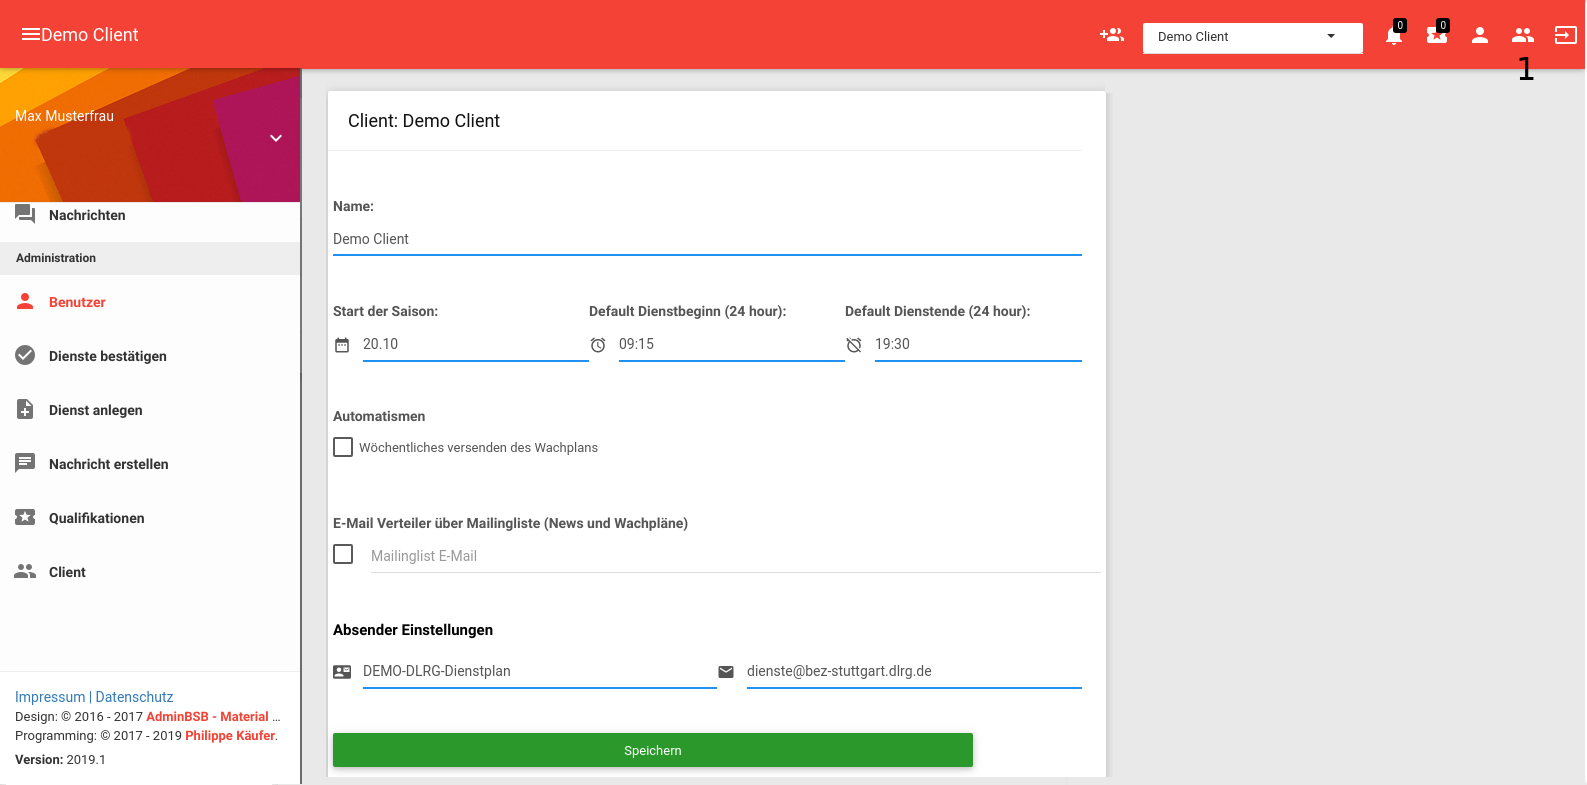
\includegraphics[width=20cm]{Bilder/view_admin.png}
	\end{addmargin} 
	\caption[Gliederungsverwaltung]{DLRG Dienstplan Gliederungsverwaltung}
	\label{fig:view_client}
\end{figure}

\section{Benutzerverwaltung}
\label{sec:admin_benutzerverwaltung}
In dem Menüpunkt Benutzer werden alle Benutzer der aktuellen Gliederung tabellarisch aufgelistet. Über diese Tabelle stehen drei Aktionen zu Verfügung:

\begin{table}[H]
	\centering
	\begin{tabular}{ll}
		
\includegraphics[width=1.5cm]{Bilder/edit.png} & Editieren der Eigenschaften eines Benutzers. \\[10pt]
		
\includegraphics[width=1.5cm]{Bilder/approve.png}	& Benutzer für die Gliederung freigeben. \\[10pt]
		
\includegraphics[width=1.5cm]{Bilder/remove.png} & Die Zuordnung des Benutzer mit der aktuellen Gliederung löschen. \\
	\end{tabular}
	%\caption{Übersicht Icons und Funktionen Benutzerverwaltung}
	%\label{fig:admin_benutzerverwaltung}
\end{table}

\section{Qualifikationsverwaltung}
\label{sec:admin_qualifikationsverwaltung}
Qualifikationen stellen die zentrale Komponente um Benutzen die Berechtigung zu erteilen, Positionen zu besetzen. Hierfür werden zunächst Qualifikationen angelegt. Darauf aufbauend sind beim anlegen eines Dienstes den einzelnen Positionen basierend auf Qualifikationen zuzuordnen. Im Dienstplan können folgend nur Benutzer, welche diese Qualifikation zugewiesen bekommen haben, sich bei entsprechenden Positionen melden. Beispiel: Zunächst wird eine Qualifikation Sanitäter angelegt. Diese Qualifikation wird Benutzern über die \ref{sec:admin_benutzerverwaltung} \nameref{sec:admin_benutzerverwaltung} zugewiesen. Werden Dienste mit Positionen \glqq Sanitäter\grqq{} angelegt, können nur entsprechende Nutzer mit der Qualifikation \glqq Sanitäter\grqq{} sich für diese Position melden.

\vspace*{5mm} \noindent Das anlegen von Qualifikationen bedingt folgende Eingaben:

\begin{itemize}
	\item[\textbf{Name:}] Name der Qualifikation.
	\item[\textbf{Abkürzung:}] Abkürzung der Qualifikation. Diese Abkürzung wird verwendet, wenn der Name für Eingabefelder, Anzeigen oder Ausdrucke zu lang ist. Es wird empfohlen hier max. 5 Zeichen zu verwenden.
	\item[\textbf{Default:}] \glqq Soll die Qualifikation bei anlegen von einem Service automatisch erstellt werden?\grqq{} Ist die Checkbox markiert, werden beim erzeugen eines Dienstes automatisch Positionen mit dieser Qualifikation angelegt.
	\item[\textbf{Default Anzahl:}] Gibt die Anzahl der Positionen an, welche beim erzeugen von Diensten automatisch angelegt werden.
	\item[\textbf{Erforderlich:}] Ist eine Position bei Diensten zwingend erforderlich, kann diese markiert werden (ref.: \ref{sec:admin_service} \nameref{sec:admin_qualifikationsverwaltung}). Diese Checkbox gibt den Standartwert vor, wenn eine Position mit dieser Qualifikation automatisch oder manuell einem Dienst hinzugefügt wird.
\end{itemize}

\begin{lamp}[frametitle={Qualifikationen Benutzern zuweisen}]
	Über die Benutzerverwaltung können Qualifikationen den Benutzern zugewiesen werden. Die Zuweisung erfolgt getrennt für jede Gliederung/Mandant. Mit dem Zuweisen werden Benutzer automatisch via E-Mail über diese Aktion informiert.
\end{lamp}

\section{Dienstverwaltung}
\label{sec:admin_service}
Dienste bestehen aus mindestens einer und beliebig vielen Positionen. Über den Menüpunkt Dienste (Kapitel \ref{cha:dienste} \nameref{cha:dienste}) werden alle angelegten Dienste der aktuellen Saison angezeigt. Das Anlegen von Diensten unterliegt den Administratoren einer Gliederung und erfolgt unter dem Menüpunkt \glqq Dienst anlegen \grqq{}. Ein Dienst hat folgende Eigenschaften:

\begin{itemize}
	\item[\textbf{Datum:}] Datum des Dienstes.
	\item[\textbf{Freigabe:}] Wenn Personen sich auf eine Position melden, müssen diese erst von einem Administrator bestätigt werden.
	\item[\textbf{Bemerkung:}] Dieses Feld kann z.B. für dem Namen einer Veranstaltung o.ä. verwendet werden. Alternativ ist dieses leer zu lassen.
	\item[\textbf{Positionen:}] Es können beliebig viele Positionen mit folgenden Eigenschaften hinzugefügt werden:
	\begin{itemize}
		\item \textbf{Qualifikation:} Definiert die Qualifikation für diese Position.
		\item \textbf{Person:} Zugewiesene Person. Beim anlegen kann dies auf \glqq -- Bitte wählen -- \grqq{} gesetzt bleiben. Soll Direkt eine Person zugewiesen werden ist diese aus dem Dropdown zu wählen. Die Liste ist nach Nachnamen sortiert, auch wenn die Anzeige den ersten Buchstabe des Vornamens mit anzeigt. Personen mit passender Qualifikation sind grün hinterlegt. Personen welche Positionen neu zugeteilt wurden, werden via E-Mail automatisch darüber in Kenntnis gesetzt.
		\item \textbf{Kommentar:} Optinales Feld für z.B. Infos wenn eine Position eine extra Sonderaufgabe zugewiesen wird oder eine andere Dienstzeit aufweist.
		\item \textbf{Erforderlich:} Ist diese Position zwingend zu besetzten oder optional? Hat Auswirkung auf die Rote Zahl der freien Dienste in der Dienstauflistung (\ref{cha:dienste} \nameref{cha:dienste}) sowie auf die Statistiken.
	\end{itemize}
\end{itemize}
Melden sich Personen selbständig für Dienste bzw. deren Positionen, werden alle Admins via E-Mail darüber in Kenntnis gesetzt. Die Freigabe erfolgt über die Admins auf der Dienste Ansicht (ref.: \ref{cha:dienste} \nameref{cha:dienste}). Eine Freigabe löst wiederum eine automatische Benachrichtigung der betroffenen Person aus.

\section{Nachrichtenverwaltung}
\label{sec:admin_news}
Verfasste Nachrichten werden an alle Nutzer versendet. Je nach Einstellung der Gliederung wird eine E-Mail an die Mailingliste oder aber an jeden Benutzer einzeln versendet.
Nachrichten werden unter dem Menüpunkt \glqq Nachrichten\grqq{} Chronologisch aufgelistet. Zusätzlich wird die neueste Nachricht auf dem Dashboard (ref.:\ref{cha:dashboard} \nameref{cha:dashboard}) dargestellt.